% !TeX encoding = UTF-8
% !TeX program = xelatex
% !TeX spellcheck = en_US

\documentclass[degree=bachelor,language=chinese,fontset = windows]{ustcthesis}
% degree    = doctor|master|bachelor
% language  = chinese|english

% 加载宏包、全部的配置
% !TeX root = ./main.tex

\ustcsetup{
  title              = {对新墨西哥州某卤水矿沉降的建模},
%  title              = {基于SBAS-InSAR技术的对新墨西哥州某卤水矿沉降的建模},
  title*             = {Modeling of a New Mexico Brine Well subsidence},
%  title*             = {Modeling of a New Mexico Brine Well subsidence, Revealed by SBAS-InSAR},
  author             = {梁康},
  author*            = {Kang Liang},
  speciality         = {地球物理学},
  speciality*        = {Geophysics},
  supervisor         = {查显杰~副教授, 路中~教授},
  supervisor*        = {Prof. Xianjie Zha, Prof. Zhong Lu},
  % date               = {2017-05-01},  % 默认为今日
  % professional-type  = {专业学位类型},
  % professional-type* = {Professional degree type},
  % secret-level       = {秘密},     % 绝密|机密|秘密,注释本行则不保密
  % secret-level*      = {Secret},  % Top secret|Highly secret|Secret
  % secret-year        = {10},      % 保密年限
  % cite-style = {inline},
}


% 加载宏包
\usepackage{graphicx}
\usepackage{booktabs}
\usepackage{longtable}
\usepackage[ruled,linesnumbered]{algorithm2e}
\usepackage{siunitx}
\usepackage{amsthm}
\usepackage{lscape}


% 数学命令
\input{math-commands.tex}

% 配置图片的默认目录
\graphicspath{{figures/}}

% 用于写文档的命令
\DeclareRobustCommand\cs[1]{\texttt{\char`\\#1}}
\DeclareRobustCommand\pkg{\textsf}
\DeclareRobustCommand\file{\nolinkurl}

% hyperref 宏包在最后调用
\usepackage{hyperref}



\begin{document}

% 研究生论文:
%   封面,原创性声明和授权使用声明
%   frontmatter: 摘要,目录,[图、表清单],[符号说明]
%   mainmatter: 正文章节,参考文献
%   appendix: 附录
%   backmatter: 致谢,已发表论文列表
%
% 本科生论文:
%   封面
%   frontmatter: 致谢,目录,摘要
%   mainmatter: 正文章节,参考文献
%   appendix: 附录

\maketitle
\copyrightpage

\frontmatter
% !TeX root = ../main.tex

\begin{acknowledgements}

在研究完成本科毕业设计期间,我有幸得到了两位老师的教导,
他们是:我的导师,中国科大查显杰副教授,美国南卫理公会大学路中教授。
两位深厚的学术功底,严谨的工作态度和敏锐的科学洞察力使我受益良多。
衷心感谢他们予我的悉心教导和热情帮助。

长安大学牛玉芬同学在建模方面给了我技术以及经验上的支持,参与了论文的修改工作,
美国南卫理公会大学王佳辉同学在InSAR数据处理方面提供很多帮助,
武汉大学韩亚坤同学,长安大学康亚同学提供了很多经验支持,
感谢他们在我完成本科毕业设计方面的热情帮助。

在科大的四年的学习生活里,我收获丰厚。
感谢科大兢兢业业的教师们,给予我最优质严谨和有启发性的教育,他们包括
汪琥庭,李娟,毛甜甜,柴松,朱晓东,郭经纬,李毅,魏渭,陶鑫,田涌波,
朱文光,胡宗好,刘斌,万柯松,文健,郑坚坚,卫国,王杰等。
感谢侯冠旺,曹炅宣,李星宇,张炜,张鉴然,陈浩铭,范文武,
崔鑫,查睿,张钰榕,周祠锦,李金涛,邓宝,李琪桦等同窗好友
以及我的室友姜化聪,张昊清,许寅超的关心与照顾。

衷心感谢我的家人、朋友,以及同学们,真是在他们的鼓励和支持下我才得以顺利完成此论文。

%最后还要感谢我的女朋友,在我21年的生命里从来没有出现,让我得以专心学习,顺利毕业。
\end{acknowledgements}

\tableofcontents
% !TeX root = ../main.tex

\ustcsetup{
  keywords = {
    SAR, InSAR, Mogi, 永久散射体干涉(PS-InSAR), 卤水井, 下沉, 建模
  },
  keywords* = {
    SAR, InSAR, Mogi, Persist Scatter Interferometry(PS-InSAR), 
    Brine well, Subsidence, Modeling
  },
}

\begin{abstract}
  大尺度的地表沉降是一种严重的灾害,随着城市的建设,地面沉降以及其所造成的次生灾害
  对城市的发展建设的危害越来越大,严重的是,这种灾害没有明显的前兆并且很难提前做出预测。
  
  本课题拟通过新墨西哥州某一塌陷卤水矿的InSAR反演的形变结果,做出沉降的物理模型。
  比较InSAR反演的模型和同一研究区域其他研究的成果,分析InSAR在解决此类问题上的优劣性,
  并对未来的InSAR技术在相关领域的作用做了展望。
\end{abstract}

\begin{enabstract}
  This is a sample document of USTC thesis \LaTeX{} template for bachelor,
  master and doctor. The template is created by zepinglee and seisman, which
  orignate from the template created by ywg. The template meets the
  equirements of USTC theiss writing standards.

  This document will show the usage of basic commands provided by \LaTeX{} and
  some features provided by the template. For more information, please refer to
  the template document ustcthesis.pdf.

\end{enabstract}

%\listoffigures
%\listoftables
%\input{chapters/notation.tex}

\mainmatter
% !TeX root = ../main.tex

\chapter{简介}

\section{研究背景和意义}

地表形变的监测是了解地球内部物理过程的重要手段。
许多地球物理现象,如火山,地震等,都会伴随地表的形变。
地表形变携带着这些现象的信息,如果能够正确地提取并使用这些信息,
会加深人类对于地球表面及内部各种物理化学演化过程的了解,
更好地服务于社会的生产和生活。

在实际应用中,地表形变的监测是了解和预防地质灾害的重要方法。
近年来,地面沉降及其引发的次生灾害对各国的经济及社会发展造成越来越严重的损失。
然而,传统的形变监测手段难以满足当前监测的要求:
传统方法需要人工在有限的点上布设台站,需要人力长期参与,且某些条件恶劣的区域很难人工操作;
由于人力成本的限制,在大尺度的范围上很难布设足够密的台站,而过于稀疏的台站并不能满足监测的需求。

合成干涉孔径雷达(Interferometric Synthetic Aperture Radar,InSAR)监测
具有成本低,覆盖范围广,全天候,非接触等优良特点。
而且相较于GPS,InSAR在垂直方向的能提供更高的精度,%\cite{knuth84}
目前已在地表沉降监测方面广泛应用,且取得了突出的成果
\cite{kimEvolutionSinkholesWink2019b,shiSubsidenceSinkholesWink2019a}。

本文通过研究一卤水井的沉降,验证了InSAR技术在研究此类现象上的有效性,
并对该区域的沉降建立物理模型,
所得的物理模型和实际导致沉降的地下空洞一致性良好,
进一步地表明InSAR技术在此类问题确实是一种有效的办法,
并且成本较低,值得我国大力推广。

\section{国内外研究现状}
由于InSAR技术在地表形变监测领域的独特优势,
在它从诞生开始受到微波遥感领域的强烈关注。
近些年来,InSAR发展出来一系列的算法,如PS(persistent scatterer)
\cite{ferrettiPermanentScatterersSAR2001,hooperNewMethodMeasuring2004},
SBAS(small baseline subsets)
\cite{berardinoNewAlgorithmSurface2002,hooperMultitemporalInSARMethod2008},
SqueeSAR\cite{ferrettiNewAlgorithmProcessing2011}
等,
能够对克服原始InSAR技术的种种劣势,
在地表形变监测领域有广泛的应用。

在1978年NASA SEASET卫星发射以后,星载SAR开始登上历史舞台并应用与地球表面研究。
关于星载干涉SAR的原理研究最早可以追溯到20世纪70年代\cite{ziskNewEarthbasedRadar1972},
InSAR的首次应用发生在上个世纪80年代末
\cite{zebkerTopographicMappingInterferometric1986,goldsteinInterferometricRadarMeasurement1987}。
1989年,Gabriel首次使用D-InSAR技术验证了InSAR技术可以在大尺度(50km)区域上检测到极小的形变(1cm或更小)
\cite{gabrielMappingSmallElevation1989},
验证了InSAR技术在沉降监测方面的可行性。

2001年,Ferretti等人首次提出PS-InSAR技术(permanent scatterer)
\cite{ferrettiPermanentScatterersSAR2001}
并将其应用与地面沉降速率的监测
\cite{ferrettiNonlinearSubsidenceRate2000}。
2004年,Hooper提出了新的PS-InSAR算法(persistent scatterer),
并将这一新的算法应用于植被茂盛的火山区域,获取了地表的形变速率
\cite{hooperNewMethodMeasuring2004},
对比发现,此PS算法的结果和GPS与水准测量的结果吻合,
大部分的PS点的可靠性较高。
2008年,Hooper将PS-InSAR和SBAS结合,
提取了更多的PS点,并进一步提高了信噪比
\cite{hooperMultitemporalInSARMethod2008}。
2011年,Ferretti等人将PS点(persistent scatterer)和DS点(distributed scatterer)
的信号结合,提出了SqueeSAR技术。

自从1991年ERS-1卫星发射,大量的SAR数据被获取,使得InSAR得到了广泛的应用。
目前InSAR技术的应用主要分为以下几个方面:
\begin{enumerate}
  \item 火山的喷发期和休眠期地表的形变可以用来研究火山结构,
  火山喷发机制,以及做火山灾害的危害性评估\cite{luInSARImagingVolcanic2007};
  \item 地震震前,震时,震后的地表形变提供了震源定位,断层几何形状,岩石破裂动力学过程;
  地壳和上地幔物理性质等研究的必要信息
  \cite{massonnetDisplacementFieldLanders1993,biggsMultiinterferogramMethodMeasuring2007};
  \item 地下水的注入和开采,矿物开采,缓慢移动的滑坡导致的形变能够为此类现象的负面性影响的评估和缓解提供数据支持
  \cite{zhangMappingGroundSurface2012,zhaoLargeareaLandslideDetection2012};
  \item 冰川移动的数据能提高人类对全球变暖以及海平面上升的认识
  \cite{rignotMassBalancePolar2002};
  \item 湿地水平面的变化可以提高对洪水灾害的认识和评估
  \cite{luRadarsat1ERSInSAR2008}。
\end{enumerate}

\section{本研究的主要内容}

\subsection{使用SBAS-InSAR技术获取当地地表形变}
本研究选取该卤水井所在区域(约1km×1km)ALOS 1(Advanced Land Observation Satellite 1)从2007年到2011年的15幅影像,
通过SBAS-InSAR技术获取当地地表形变以及平均的形变速率。这一步使用的软件为StamPS\cite{hooperMultitemporalInSARMethod2008}。


\subsection{使用Mogi模型对该形变建模}
首先观察SBAS-InSAR得到的形变特征,选取比较合适的Mogi\cite{mogiRelationsEruptionsVarious1958}模型,对该形变进行理论建模,
建模所使用的软件为GBIS\cite{bagnardiInversionSurfaceDeformation2018}。
然后与已有的研究成果相对比,并结合当地地质背景,分析所得模型的可靠程度。

本研究的组织结构如图\ref{fig:flow}所示。
\begin{figure}[htb]
  \centering
  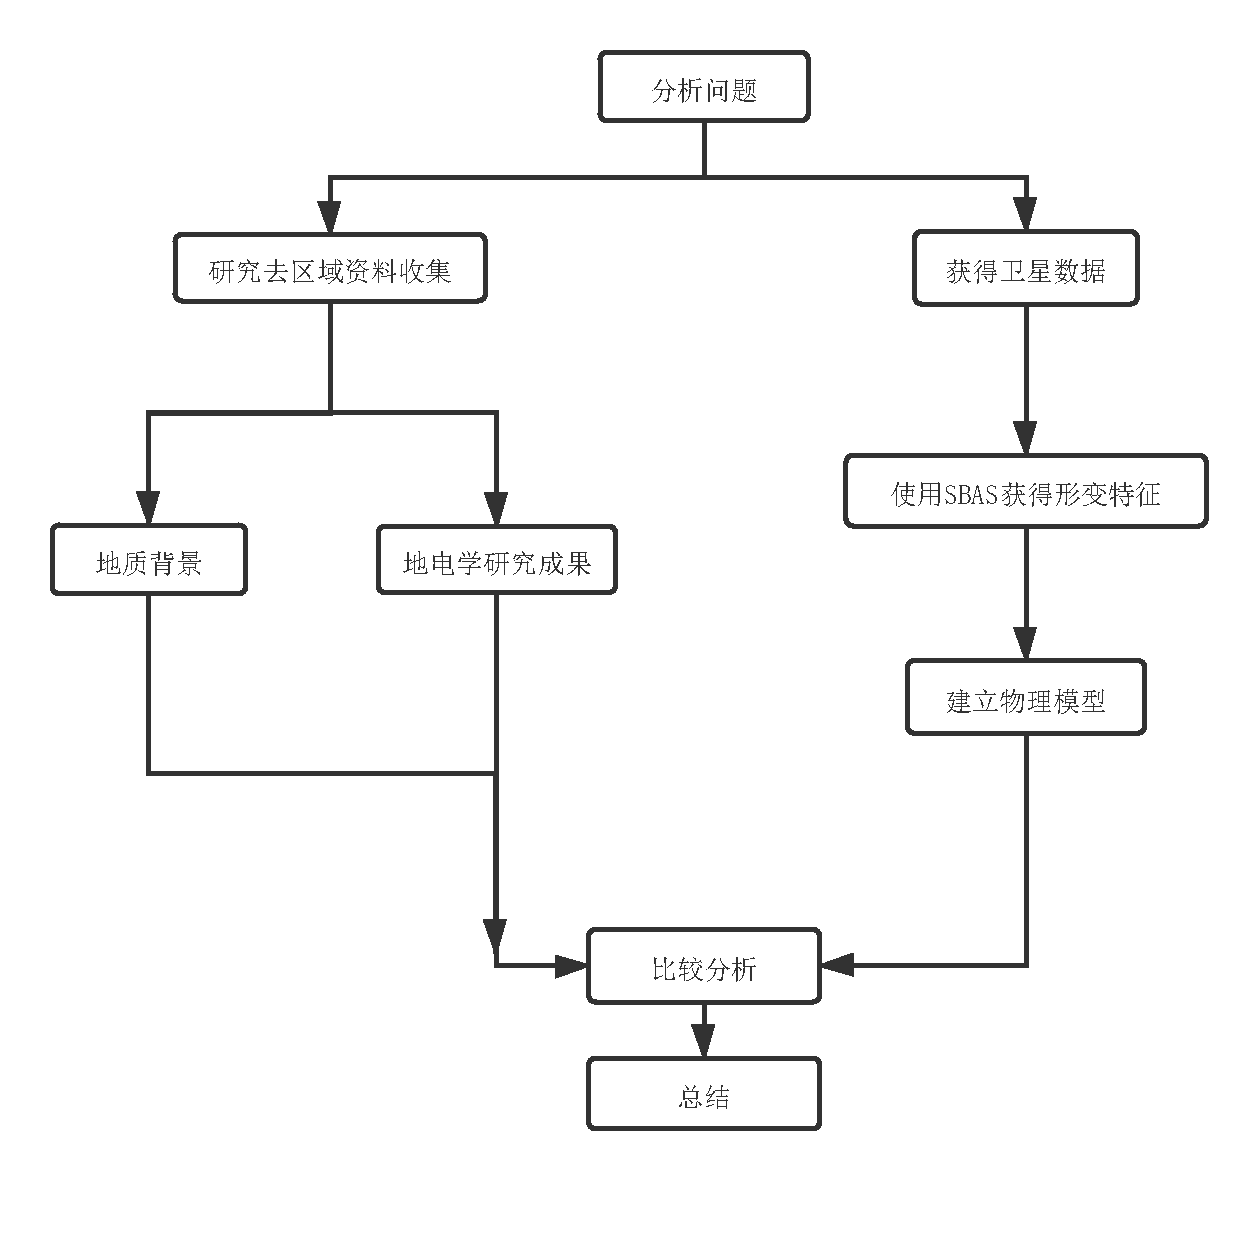
\includegraphics[width=\textwidth]{flow.pdf}
  \caption{本研究的组织结构}
  \label{fig:flow}
\end{figure}
\chapter{InSAR技术原理}

\section{SAR与InSAR原理}

\subsection{SAR}

SAR由传统的雷达技术发展而来。
通过水平向和垂直向的压缩成像技术能够实现以较小的雷达天线
得到较高空间分辨率的影像。
每幅SAR影像的数据为光波从天线到地面每一个像素点然后反射再被天线接受的相位延迟。
即
\begin{equation}
    \phi=-\frac{4\pi}{\lambda}r
\end{equation}

\subsection{InSAR}

如果对于同一块区域有两幅影像,就可以对两幅影像做干涉处理。
原理如图\ref{fig:geometry}所示。
\begin{figure}[htb!]
    \centering
    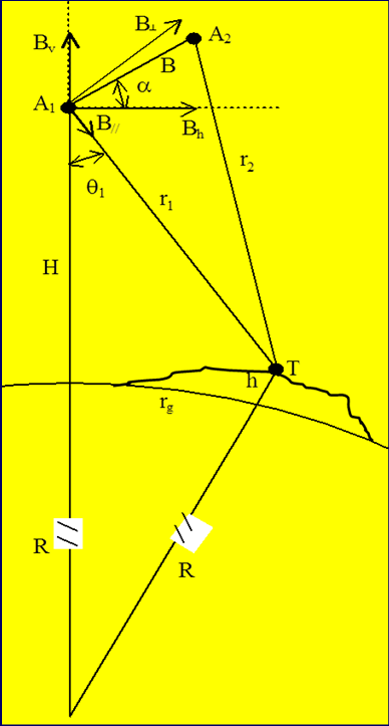
\includegraphics[width=0.5\textwidth]{geometry.png}
    \caption{InSAR技术原理示意图}
    \label{fig:geometry}
\end{figure}
所谓干涉,就是指二者相位相减。即
\begin{equation}
    \Delta \phi=-\frac{4\pi}{\lambda}(r_1-r_2)
\end{equation}
其中$\Delta r$为卫星视线方向的变化。
注意这里讨论的只是忽略大气效应即其他失相干效应,只考虑理想情况。
通常情况下,两幅影像并不是在相同的位置拍摄,二者之间有一定的距离。
所以当不存在任何的地表形变的情况下,可以通过一些几何的参数将此变化表达出来。
\begin{equation}
    \Delta \phi=\frac{4\pi}{\lambda}\left(\sqrt{r_1^2−2(B_hsinθ_1−B_{\perp}sinθ_1)r_1+B^2}−r_1\right)
\end{equation}

如果已知数字高程模型的话,可以算出来在理想条件下,无形变时的相位差。
将实际算得的相位差和无形变时理论计算的相位差相减,剩余的相位差即为因形变引起的相位差。
\begin{equation}
    \Delta \phi_{r}=-\frac{4\pi}{\lambda}u_{LOS}
\end{equation}
其中,$u_{LOS}$为地表形变在卫星视线(line-of-site:LOS)方向的投影,
从而可以把地表在卫星视线方向的形变算出来。
这种技术称之为D-InSAR。

注意,实际的到的相位是“缠绕”的相位,即相位是处于$(-\pi,\pi]$之间的。
将缠绕的相位通过解缠操作之后才得到上文中使用的相位。
解缠的方法很多,基本的假设是相邻像素的相位差不超过$\pi$。

诸多实例(火山喷发变形,地震震前和震后变形,地面沉降)
均证明InSAR是一种有效的测量地表形变的技术。
\section{PS-InSAR简介}

两幅SAR影像间隔时间可能很长,如果地表有植被,或者一年中有部分时间被冰雪覆盖,
地表散射体在这段时间内有较大的变化,有可能导致干涉图的失相干。
如果能挑出地表散射体中较稳定的部分,如建筑物,道路桥梁,岩石等
永久散射体(persist scatterer)反射波的相位差,剔除掉不稳定的散射体反射波的相位差,
经相位解缠之后就能得到较可靠形变结果。
这正是PS-InSAR技术的初衷。

2001年,Ferretti等人首次提出PS-InSAR技术。
即在一组时间序列SAR影像中选取相干性和稳定性均较好的永久散射体。
通过这些PS点的相位信息获得地表形变信息。
2004年,Andy hopper提出了新的PS算法,并将其实现在StamPS软件中。
本研究使用这一软件获得形变信息。

PS-InSAR技术的主要内容为PS点的选取,分为两个步骤:
\begin{enumerate}
    \item 初步筛选。
    这一步通过分析模长的稳定性做筛选。
    Ferretti等人证明了,对于反射波的复信号,当相位的标准差较小时,有
    \begin{equation}
        \sigma_\varphi \approx \frac{\sigma_a}{\mu_a}
    \end{equation}
    其中,$\sigma_\varphi$是相位标准差,$\sigma_a$是模长的标准差,$\mu_a$是模长的均值。
    通过设置$\frac{\sigma_a}{\mu_a}$的上界$D_A$,筛选出一批PS点。
    \item 再次筛选。
    这一步通过分析相位的稳定性来做筛选。
    首先通过相位滤波得到噪声相位,对噪声相位做进一步的筛选选出最终的PS点。
\end{enumerate}

PS-InSAR的输入数据为连续的$M$幅SAR影像以及数字高程模型(DEM)。
首先,选取某一幅影像为主影像,然后通过配准,差分干涉,
以及PS点的选取等操作得到$M-1$幅干涉图,
之后通过相位解缠得到形变图以及平均形变速率图。

\section{SBAS-InSAR简介}
SBAS是另外一种利用多个SAR影像数据的时间序列InSAR方法。
SBAS通过设置选取SAR影像配对的时空基线的上限,
将所有的SAR影像分为了不同组,每组的基线较小,从而避免了空间上的失相干性,减小了失相干和高程模型误差的影响。

这里有必要简要叙述一下SBAS处理数据的算法。
假设一共有$n+1$景SAR影像数据,获取的时间分别为$t_0,t_1,\ldots,t_n$。
选取某一景影像为超级主影像。
满足时空基线限制的影响对共有$M$对。分别为$(A_1,B_1),(A_2,B_2),\ldots,(A_M,B_M)$。
则
\begin{equation}
    \Delta\phi_j=\phi_{A_j}-\phi_{A_j}
\end{equation}
其中,$j=1,2,\ldots,M$,$\phi_j$为第$j$景影像相对于超级主影像的差分相位,
$\Delta\phi_j$为第$j$组影像对的差分干涉相位,共计$M$个方程。
由已知的$\phi$根据以上方程求得$\Delta\phi$,
然后由得到的$\Delta\phi$反过来求$\phi$。
由于共有$M$个方程,$n$个未知数,方程组有无穷多组解,使用最小二乘法求最小二范数的解。

\section{本研究所用的方法}
D-InSAR在监测地面沉降方面取得了一定的成果,但由于这种方法受失相干的影响比较严重,
并不适合本研究使用。
且由于数据较少的缘故,本研究采用数据利用率更高的SBAS-InSAR方法处理数据。

\chapter{一种建模的贝叶斯方法}
\label{ch:pm}
\section{方法简介}
本研究使用GBIS\cite{bagnardiInversionSurfaceDeformation2018}作为建模软件,
此软件的建模方法为Marco Bagnardi等人提出的一种建模的贝叶斯方法。

一般的反演算法通过求解误差函数的最小值来得到最优的模型参数。
这样的方法只能给出最终的结果,无法全面或正确地得到反演参数不确定度,
所以对反演结果的可靠程度所知甚少,有得到错误的反演结果的风险。
实际上,由于反演的不唯一性,很多时候不同的参数可能对观测的结果都能做出合理的解释。
这就需要事先对反演参数可能的区间有一定的了解。

这种贝叶斯方法的特色在于能够估计并利用数据的不确定度,
通过多种统计学方法(如点估计,区间估计等),
得到所要反演参数的联合与条件后验概率分布。
实际计算机计算时,GBIS使用马尔可夫链蒙特卡洛(Markov Chain Monte Carlo)方法
以及梅特罗波利斯-黑斯廷斯(Metropolis–Hastings algorithm)算法
\cite{hastingsMonteCarloSampling1970,mosegaardMonteCarloSampling1995}
得到采样化的后验概率分布。

当前版本的GBIS软件可以通过InSAR数据和GPS数据来反演形变源的参数。
该软件自带不同几何形状的形变源的解析模型,比如
点源\cite{mogiRelationsEruptionsVarious1958},
有限球源\cite{mctigueElasticStressDeformation1987},
扁长椭球源\cite{yangDeformationInflationDipping1988},
硬币形窗台状源(penny-shaped sill-like source)\cite{fialkoDeformationDuePressurized2001},
开口一致的下沉堤坝(dipping dike with uniform opening)\cite{okadaSurfaceDeformationDue1985},
均匀滑动的断层(dipping faults with uniform slip)\cite{okadaSurfaceDeformationDue1985}。
这些解析模型均处于各项同性弹性半空间中。
其他此软件不含有的模型也可以很容易地在这套框架下实现。

\section{方法原理}

贝叶斯方法视参数$\mathbf{m}$为随机变量,数据$\mathbf{d}$为随机变量的取样。
二者的关系为
\begin{equation}
    \mathbf{d}=\mathbf{G}(\mathbf{m})+\vepsilon
\end{equation}
其中,$\mathbf{G}$为模型函数,$\vepsilon$为人为引入的误差随机变量。
由贝叶斯公式,有
\begin{equation}
    \label{eq:pm:bayes}
    P(\mathbf{m}|\mathbf{d})=\frac{P(\mathbf{d}|\mathbf{m})P(\mathbf{m})}{P(\mathbf{d})}
\end{equation}
其中$P(\mathbf{m})$为先验概率,其分布由其他方法获得。
$P(\mathbf{d})$为归一化因子。
假设$\vepsilon$服从均值为$0$,方差为$\Sigma_{\mathbf{d}}$的高斯分布,则
\begin{equation}
    \label{eq:pm:likelihood}
    P(\mathbf{d}|\mathbf{m})=(2\pi)^{\frac{N}{2}}|\Sigma_{\mathbf{d}}|^{-\frac{1}{2}}
    \exp\left(-\frac{1}{2}(\mathbf{d-Gm})^{\top}\Sigma_{\mathbf{d}}^{-1}(\mathbf{d-Gm})\right)
\end{equation}
其中$\Sigma_{\mathbf{d}}$由形变数据估计得。
这种方法旨在求得最优的模型参数$\mathbf{m}$的后验概率分布$p(\mathbf{m}|\mathbf{d})$。
下面简述算法。
\begin{enumerate}
    \item 为了节省时间,对数据$\mathbf{d}$进行采样,并估计数据的方差$\Sigma_{\mathbf{d}}$,
    具体的做法是人为选择一块没有认为没有形变的区域,通过这块区域形变数据的方差估计$\Sigma_{\mathbf{d}}$。
    \item 给定参数$\mathbf{m}$的可能区间和先验概率和循环的起始点$\mathbf{m_0}$。
    \item 由起始点$\mathbf{m_0}$计算理论形变$\mathbf{d}_0$。
    \item 由公式\ref{eq:pm:bayes}和公式\ref{eq:pm:likelihood}算得当前后验概率$p(\mathbf{m}|\mathbf{d}_i)$。
    \item 模型参数按照一定的方法随机取下一步的值,重复上一步操作,得到新的后验概率$p(\mathbf{m}|\mathbf{d}_{i+1})$。
    \item 若$p(\mathbf{m}|\mathbf{d}_{i+1})>p(\mathbf{m}|\mathbf{d}_i)$,则保留新的参数,否则放弃这一步。
          然后循环上述内容直到循环终止。
\end{enumerate}

\chapter{基于SBAS-InSAR技术的地表形变检测}

\section{研究区域}

研究区域为卡尔斯巴德未坍塌的卤水井。如图\ref{fig:studyarea}中方框所圈的内容所示。
\begin{figure}[htb]
    \centering
    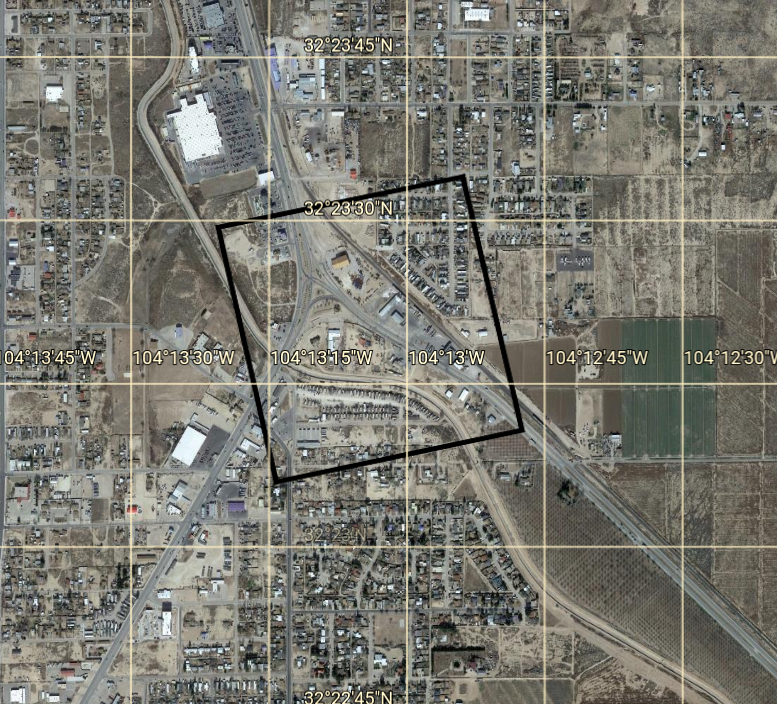
\includegraphics[width=0.8\textwidth]{studyarea.png}
    \caption{研究区域示意图}
    \label{fig:studyarea}
\end{figure}

\section{数据源}

本研究使用的数据为ALOS PALSAR的数据。
ALOS是日本与2006年发射的卫星,PALSAR为该卫星上搭载的L波段的合成孔径雷达。
数据的基本参数见表\ref{tab:palsar}。
% \begin{table}[htb]
%     \centering\small
%     \caption{数据基本参数}
%     \label{tab:palsar}
%     \begin{tabular}{@{}cc@{}}
%     \toprule
%     参数           & 值                                \\ 
%     \midrule
%     雷达           & ALOS PALSAR                      \\
%     中心频率         & 1270 MHz(L波段)                    \\
%     range方向采样数   & 94                               \\
%     azimuth方向采样数 & 252                              \\
%     heading      & $-10.13^{\circ}$至$-10.18^{\circ}$ \\
%     入射角          & $38.73^{\circ}$左右  \\
%     \bottomrule
%     \end{tabular}
% \end{table}
监测时间从2006年12月到2011年2月共计15幅影像,详情参见表\ref{tab:timeseries}。
% \begin{table}[htb]
%     \centering\small
%     \caption{数据时间序列}
%     \label{tab:timeseries}
%     \begin{tabular}{@{}cccc@{}}
%     \toprule
%     序号 & 成像时间 & 序号 & 成像时间\\ 
%     \midrule
%     1 & 2006.12.20 & 9 & 2010.05.15 \\
%     2 & 2007.06.22 & 10 & 2010.06.30 \\
%     3 & 2007.12.23 & 11 & 2010.08.15 \\
%     4 & 2008.05.09 & 12 & 2010.09.30 \\
%     5 & 2008.06.24 & 13 & 2010.11.15 \\
%     6 & 2008.12.25 & 14 & 2010.12.31 \\
%     7 & 2009.12.28 & 15 & 2011.02.15 \\
%     8 & 2010.05.30 & & \\
%     \bottomrule
%     \end{tabular}
% \end{table}
\begin{table}
    \centering\small
    \begin{minipage}{0.49\textwidth}
        \centering
    \caption{数据基本参数}
    \label{tab:palsar}
    \begin{tabular}{@{}cc@{}}
    \toprule
    参数           & 值 \\ 
    \midrule
    雷达           & ALOS PALSAR  \\
    中心频率         & 1270 MHz(L波段) \\
    range方向采样数   & 94  \\
    azimuth方向采样数 & 252  \\
    range方向像素距离 & 4.684257m \\
    azimuth方向像素距离 & 3.151791m \\
    heading      & $-10.13^{\circ}$至$-10.18^{\circ}$ \\
    入射角          & $38.73^{\circ}$左右  \\
    \bottomrule
    \end{tabular}
    \end{minipage}
    \begin{minipage}{0.49\textwidth}
        \centering
        \caption{数据时间序列}
        \label{tab:timeseries}
        \begin{tabular}{@{}cccc@{}}
        \toprule
        序号 & 成像时间 & 序号 & 成像时间\\ 
        \midrule
        1 & 2006.12.20 & 9 & 2010.05.15 \\
        2 & 2007.06.22 & 10 & 2010.06.30 \\
        3 & 2007.12.23 & 11 & 2010.08.15 \\
        4 & 2008.05.09 & 12 & 2010.09.30 \\
        5 & 2008.06.24 & 13 & 2010.11.15 \\
        6 & 2008.12.25 & 14 & 2010.12.31 \\
        7 & 2009.12.28 & 15 & 2011.02.15 \\
        8 & 2010.05.30 & & \\
        \bottomrule
        \end{tabular}   
    \end{minipage}
\end{table}
\section{数据处理}
本研究首先使用gamma软件进行干涉对的选择,选取2009年12月28日的影像为主影像,
结果如图\ref{fig:bprep}所示。
\begin{figure}[htb]
    \centering
    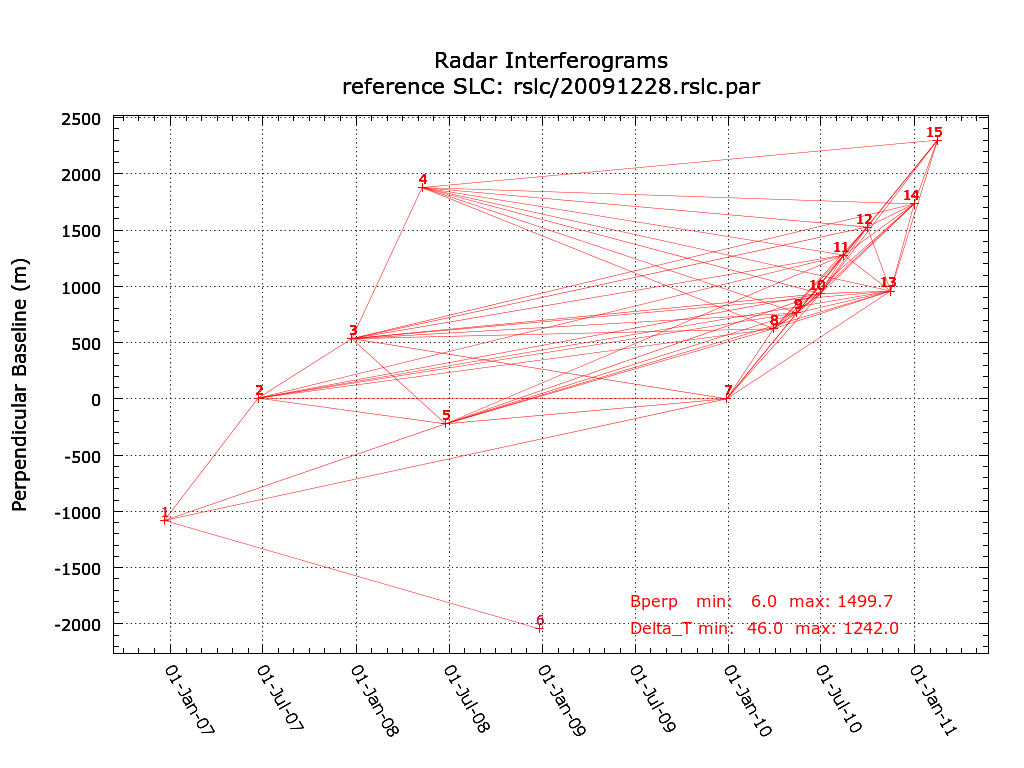
\includegraphics[width=0.8\textwidth]{bperp.png}
    \caption{时空基线连接图}
    \label{fig:bprep}
\end{figure}
然后使用StamPS软件进行SBAS技术数据处理。
处理所得平均速度如图\ref{fig:sbasv},相对的形变如图\ref{fig:sbasu}所示。
\begin{figure}[htb]
    \centering
    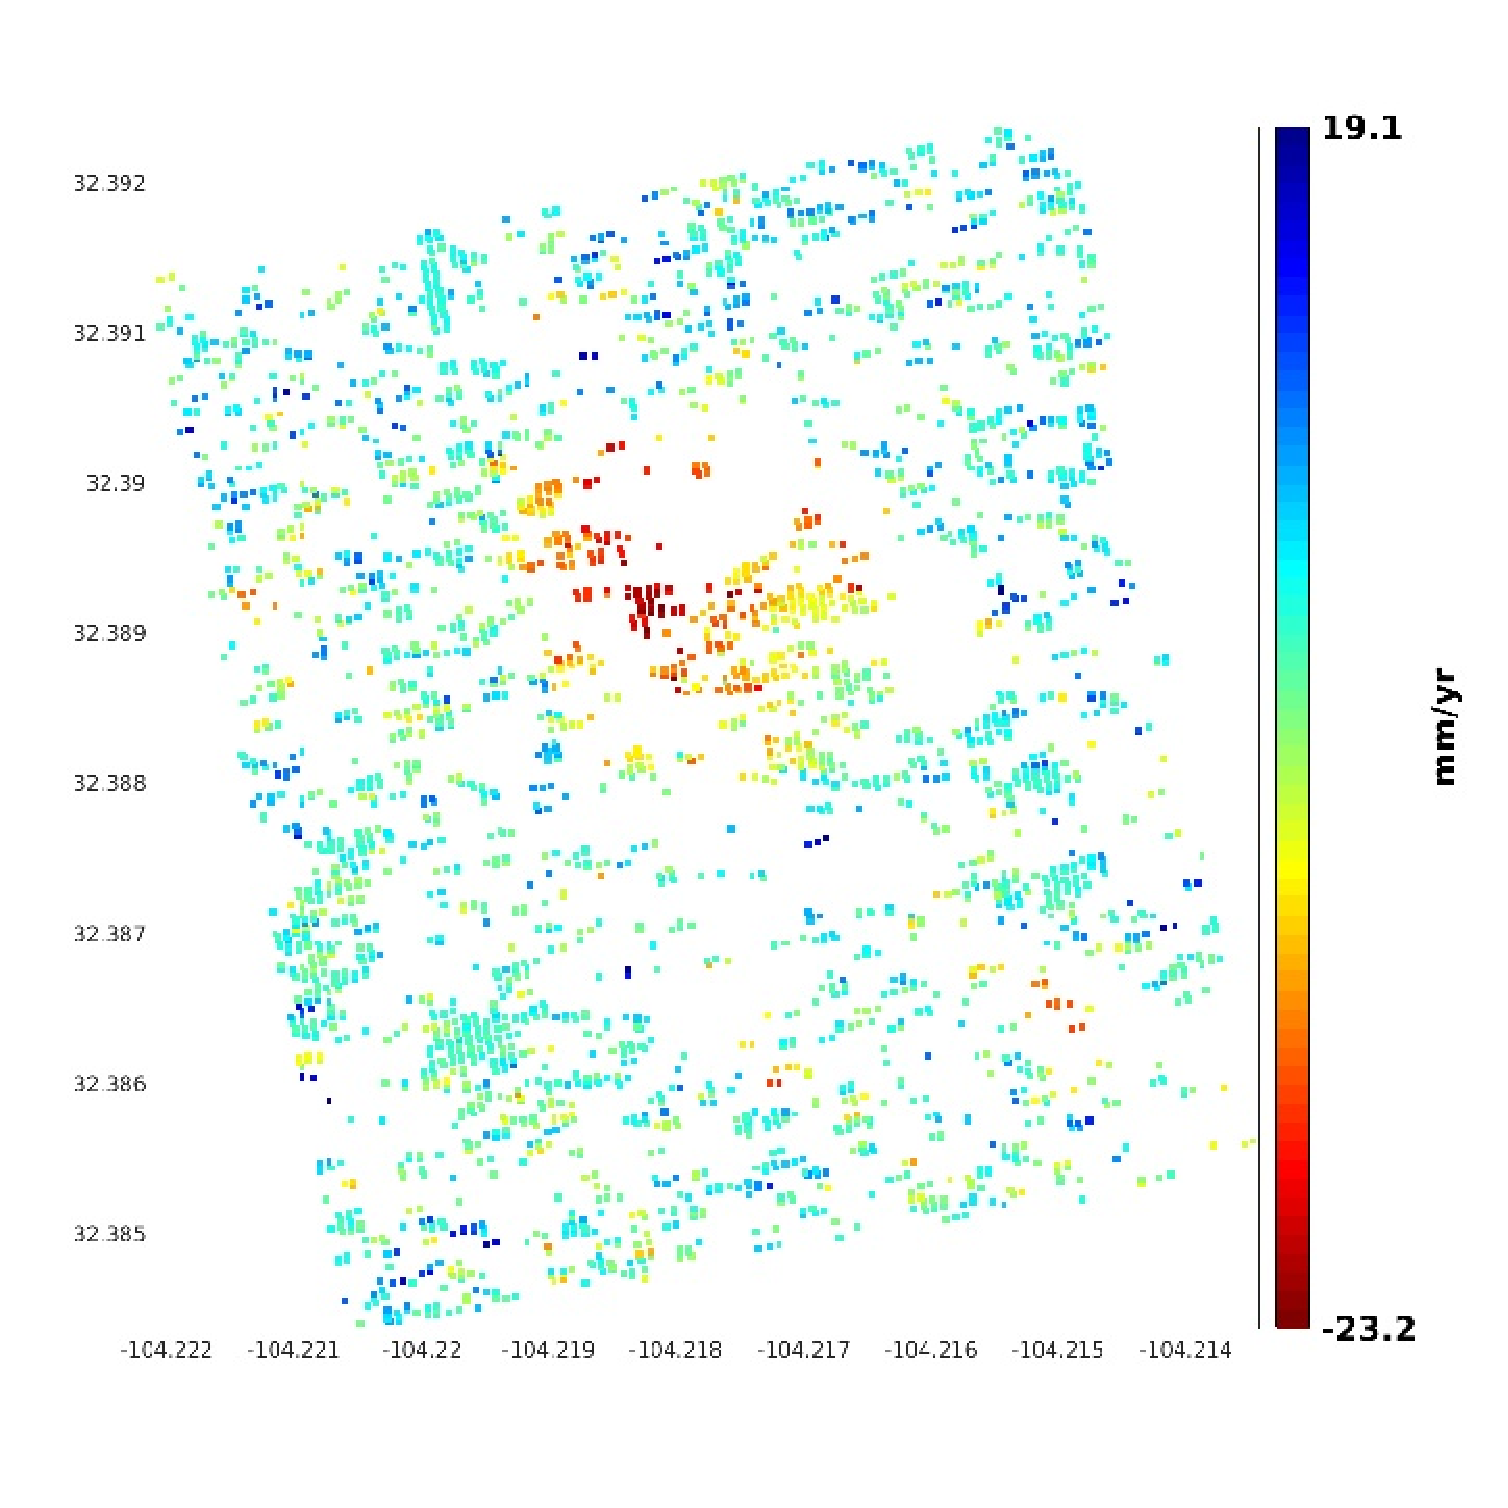
\includegraphics[width=1.0\textwidth]{sbasv.eps}
    \caption{研究区域平均沉降速率图}
    \label{fig:sbasv}
\end{figure}
\begin{figure}[htb]
    \centering
    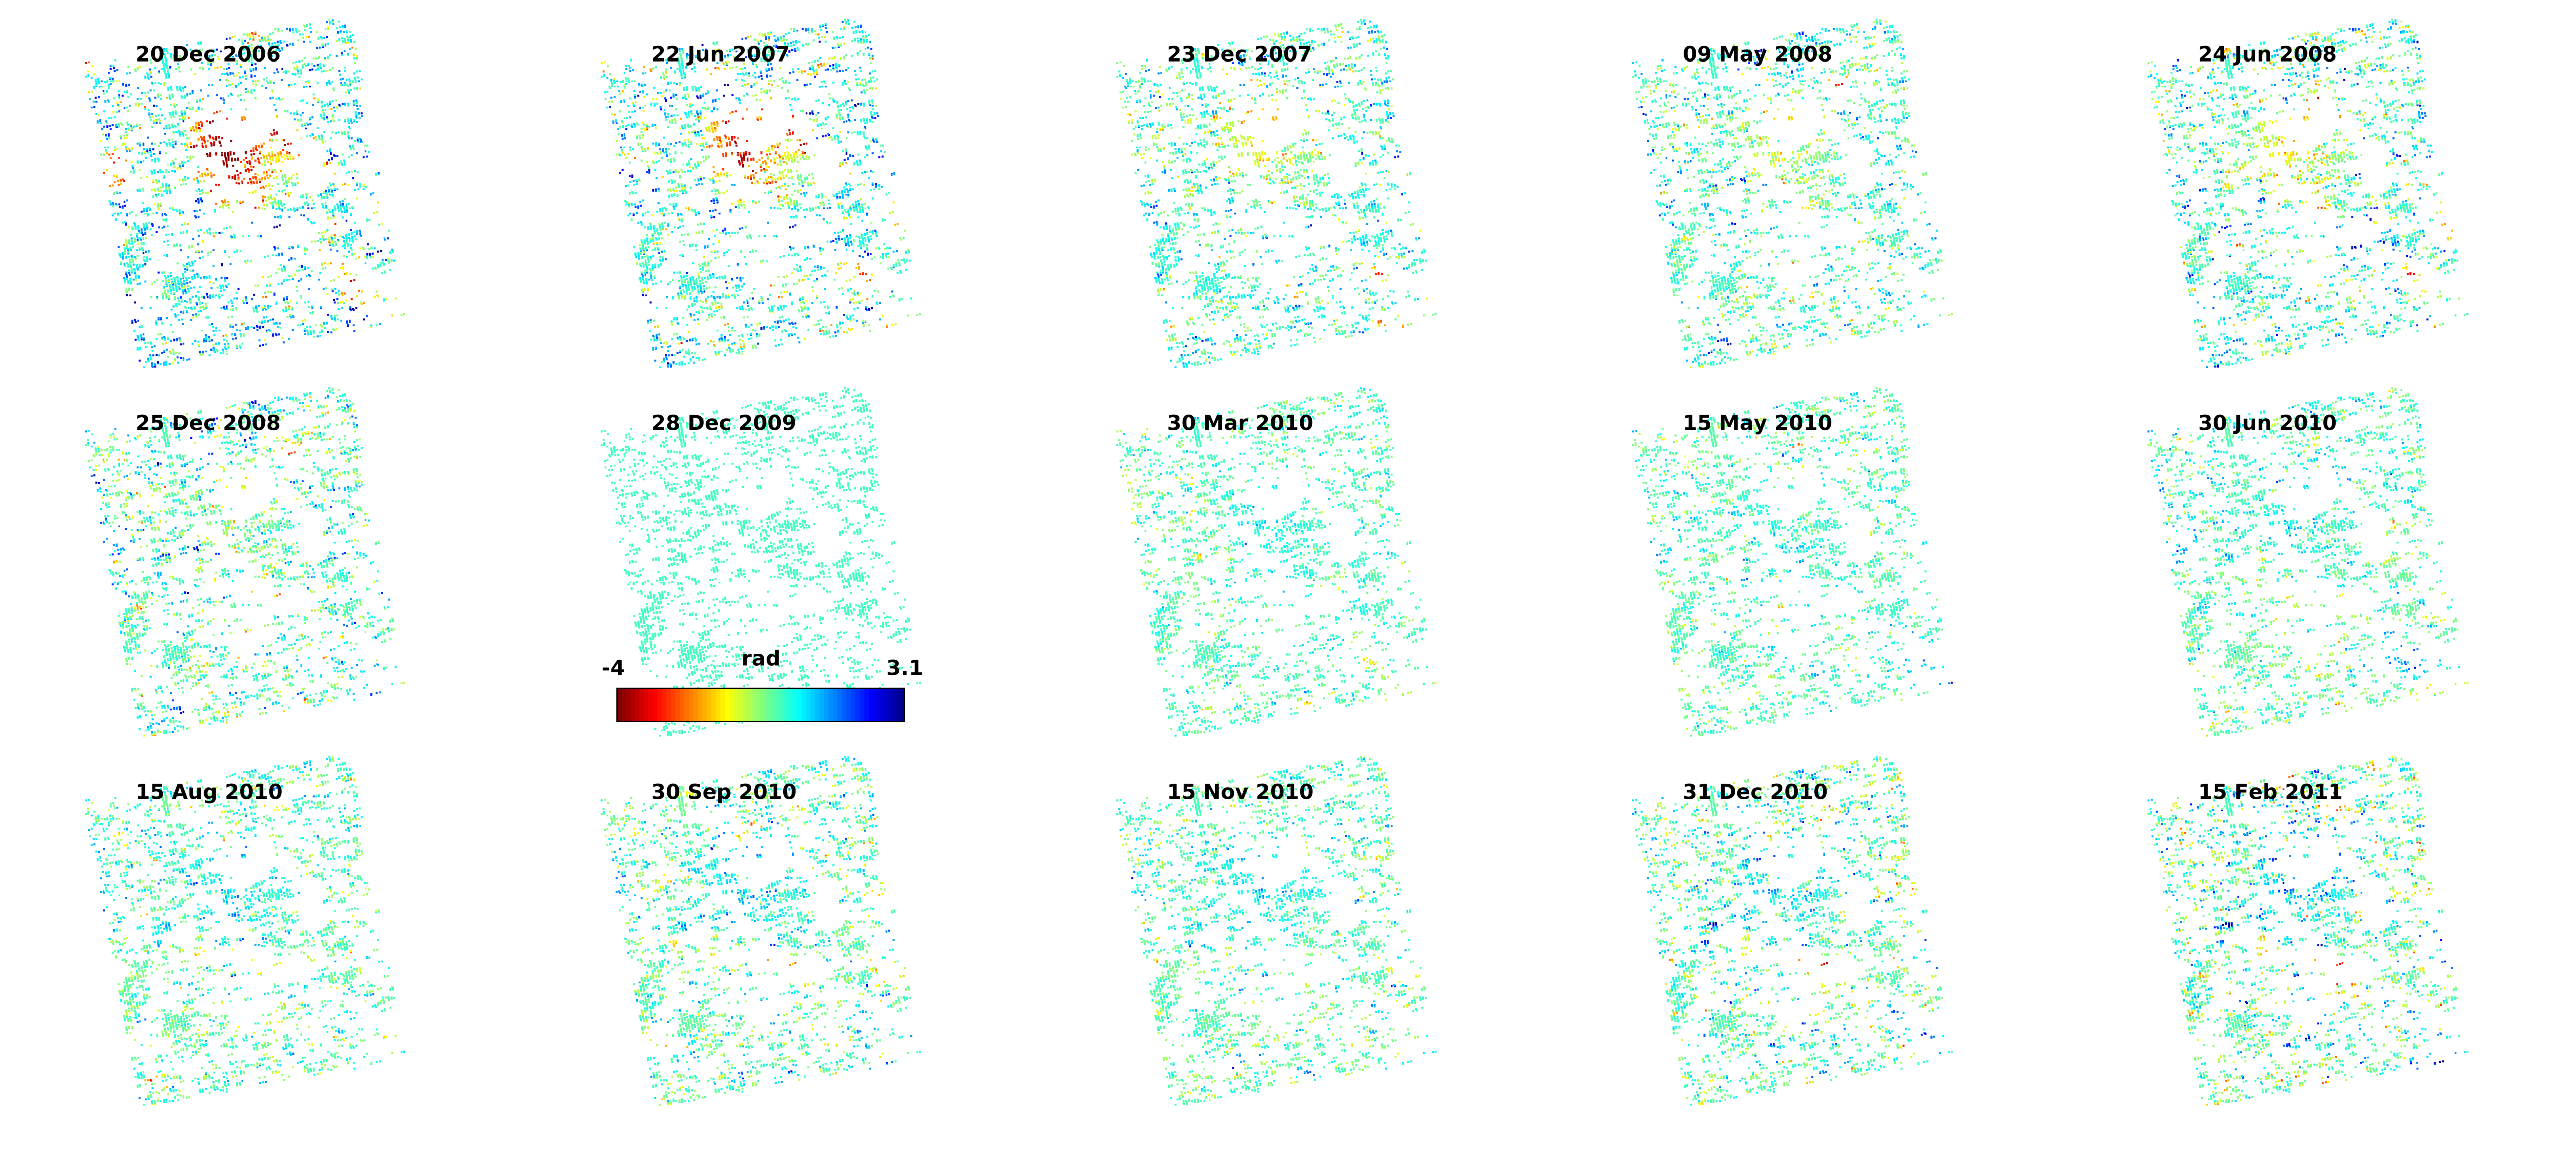
\includegraphics[width=1.0\textwidth]{sbasu.pdf}
    \caption{研究区域相对于主影像形变图}
    \label{fig:sbasu}
\end{figure}

\section{形变结果的初步分析}
从图\ref{fig:sbasv}和图\ref{fig:sbasu}中可以明显地看出中部区域有明显的沉降。
变形最明显的区域的形变可以达到平均23.2mm/year的速度,
累计最大形变可达81mm。
从形变的结果来看,此变形比较类似于点源引起的变形,该点源的位置大概在尤金妮娅1号所在的位置,
初步估计此处的沉降是尤金妮娅1号的开采导致的地下空洞引发的次生灾害。
同时,右下角部分有一定的形变,但由于在该部位所选取的PS点较少的缘故,该区域的形变很难建模。
下一步的研究将使用点源对形变做一个物理模型并分析模型和实际空洞的差别。
\chapter{针对形变的理论建模}

\section{使用数据}
使用上一章得到的平均形变速率作为建模的输入数据,
对于该区域中部的明显形变采用mogi模型建模。

\section{mogi模型}
mogi模型为最常用的点源模型。
它的基本假设为:
\begin{enumerate}
    \item 介质为各项同性线性弹性介质,可以用剪切模量$\mu$和泊松比$\nu$完全表征介质的特性。
    \item 研究空间为半空间。
    \item 扰动源为点源,即源的尺度远小于模型的尺度:$\alpha \ll d$。
\end{enumerate}

由以上基本假设可以得知,mogi模型的参数分为两个部分:
\begin{enumerate}
    \item 扰动源的参数:扰动源的位置$X,Y,Z$,以及表征扰动大小的体应变$DV$。
    \item 介质的参数:剪切模量$\mu$和泊松比$\nu$。
\end{enumerate}
其中地球介质的参数波动不大,一般设成已知量,对反演的结果影响不大。
主要的反演参数为扰动源的四个参数。

\section{建模软件}
本研究使用的建模软件为GBIS,关于反演算法和软件已经在第\ref{ch:pm}章中说明。

\section{反演过程和结果}
为了节省运算时间,首先对数据进行quadtree重采样,
采样前后的对比如图\ref{fig:unsample}和\ref{fig:subsample}所示。
\begin{figure}[htp]
    \centering
    \begin{minipage}{0.9\textwidth}
        \centering
        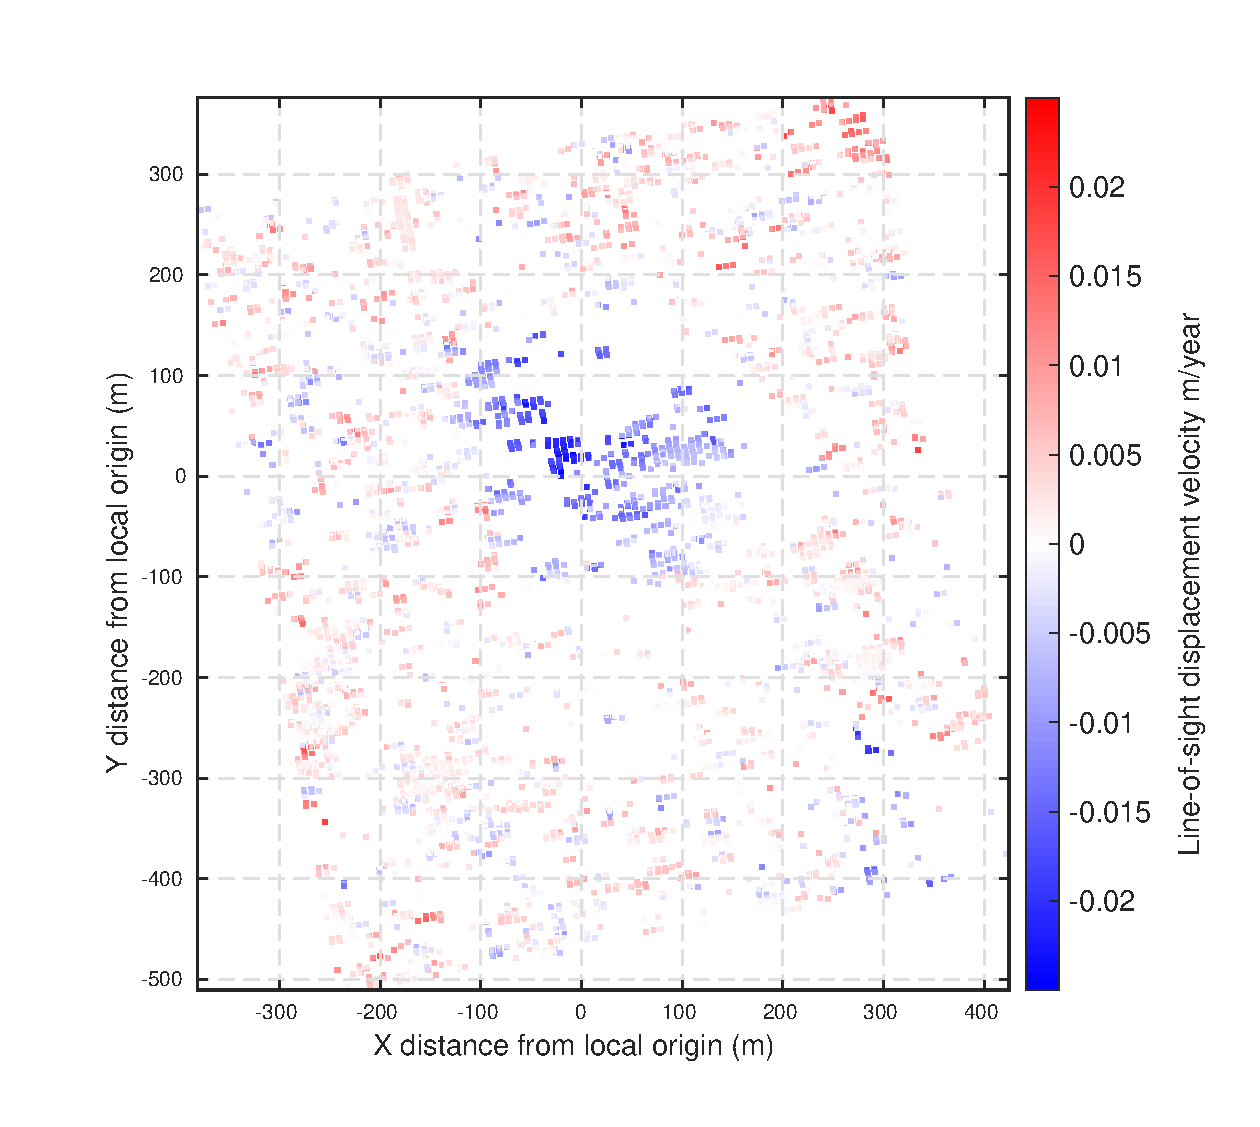
\includegraphics[width=0.8\textwidth]{unwrapped.eps}
        \caption{原始形变图}
        \label{fig:unsample}
    \end{minipage}
    \qquad
    \begin{minipage}{0.9\textwidth}
        \centering
        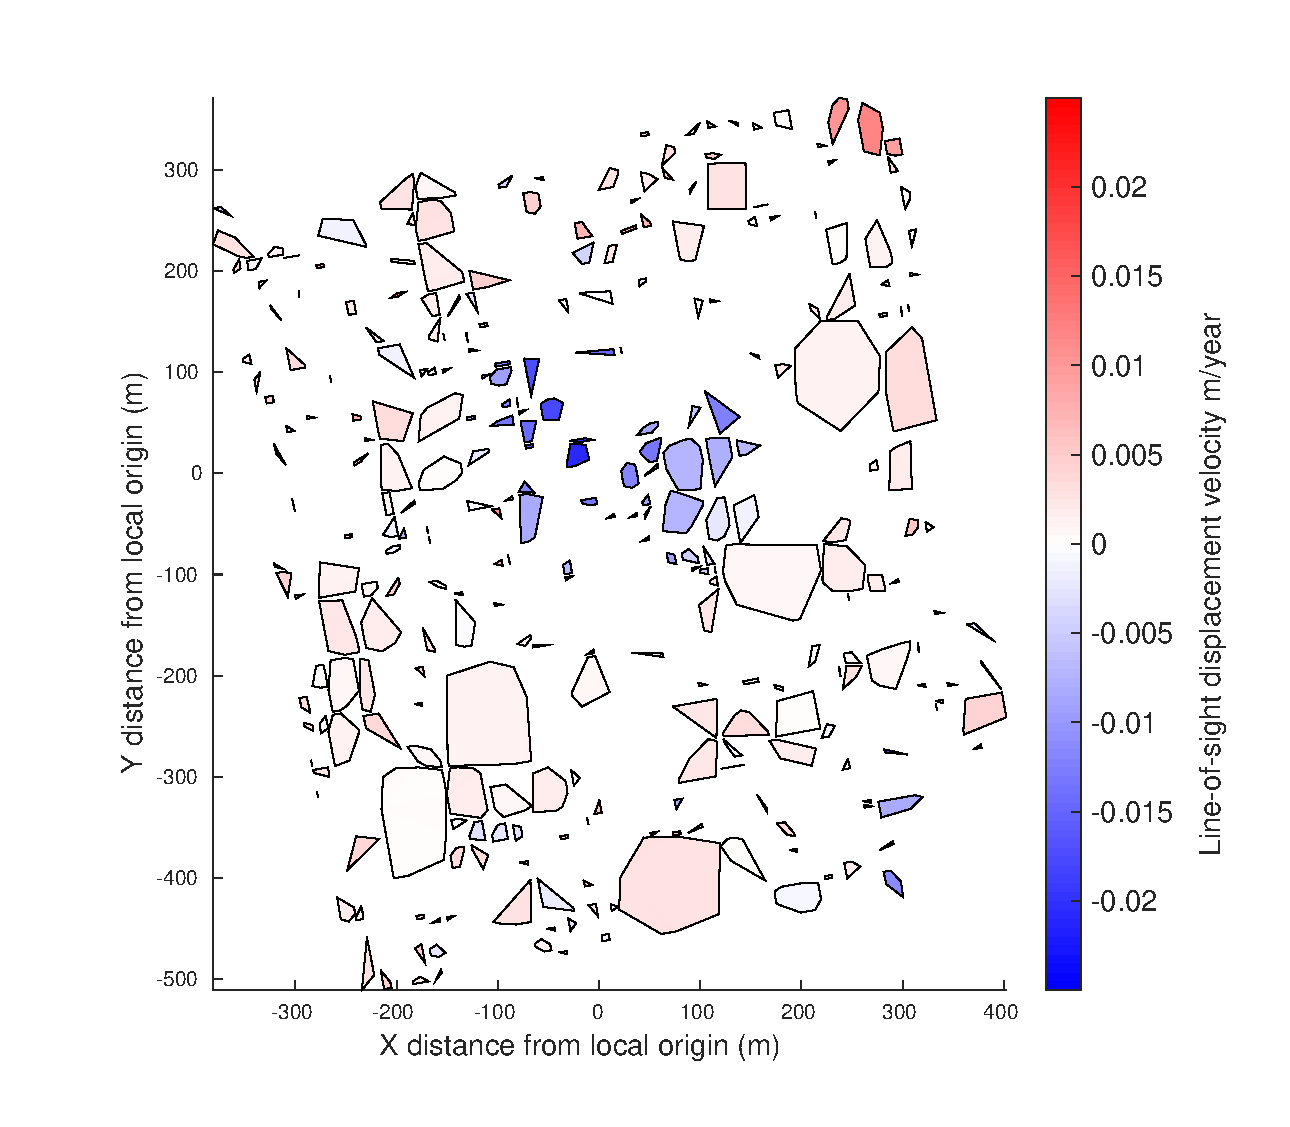
\includegraphics[width=0.8\textwidth]{subsampled.eps}
        \caption{quadtree采样后的形变图}
        \label{fig:subsample}
    \end{minipage}
%    \caption{aaa}
%    \label{zhong}
\end{figure}
然后开始反演。反演的结果见表\ref{tab:modelpar}。
\begin{table}[htb]
    \centering\small
    \caption{模型参数}
    \label{tab:modelpar}
    \begin{tabular}{@{}cccccc@{}}
    \toprule
    参数       & 最优值 & 平均值 & 中位值 & 2.5\% & 97.5\% \\ 
    \midrule
    mogi X    & -14.20 & -13.19 &-12.59 & -50.51 & 10.94 \\
    mogi Y     & 45.89 & 46.84 & 46.34 & 18.01 & 78.61\\
    mogi depth & 103.57 & 114.46 & 105.80 & 85.44 & 238.95\\
    mogi DV   & -1121.93 & -1240.33 & -1111.70 & -3228.15 & -713.27\\
    InSAR 常数 & 0.00 & 0.00 & 0.00 & -0.00 & 0.01\\
    \bottomrule
    \end{tabular}
\end{table}
参数的后验概率见图\ref{fig:pdf}。
从该图中可以看出,X,Y的后验概率分布比较散,这两个参数的收敛性较差。
\begin{figure}[htb]
    \centering
    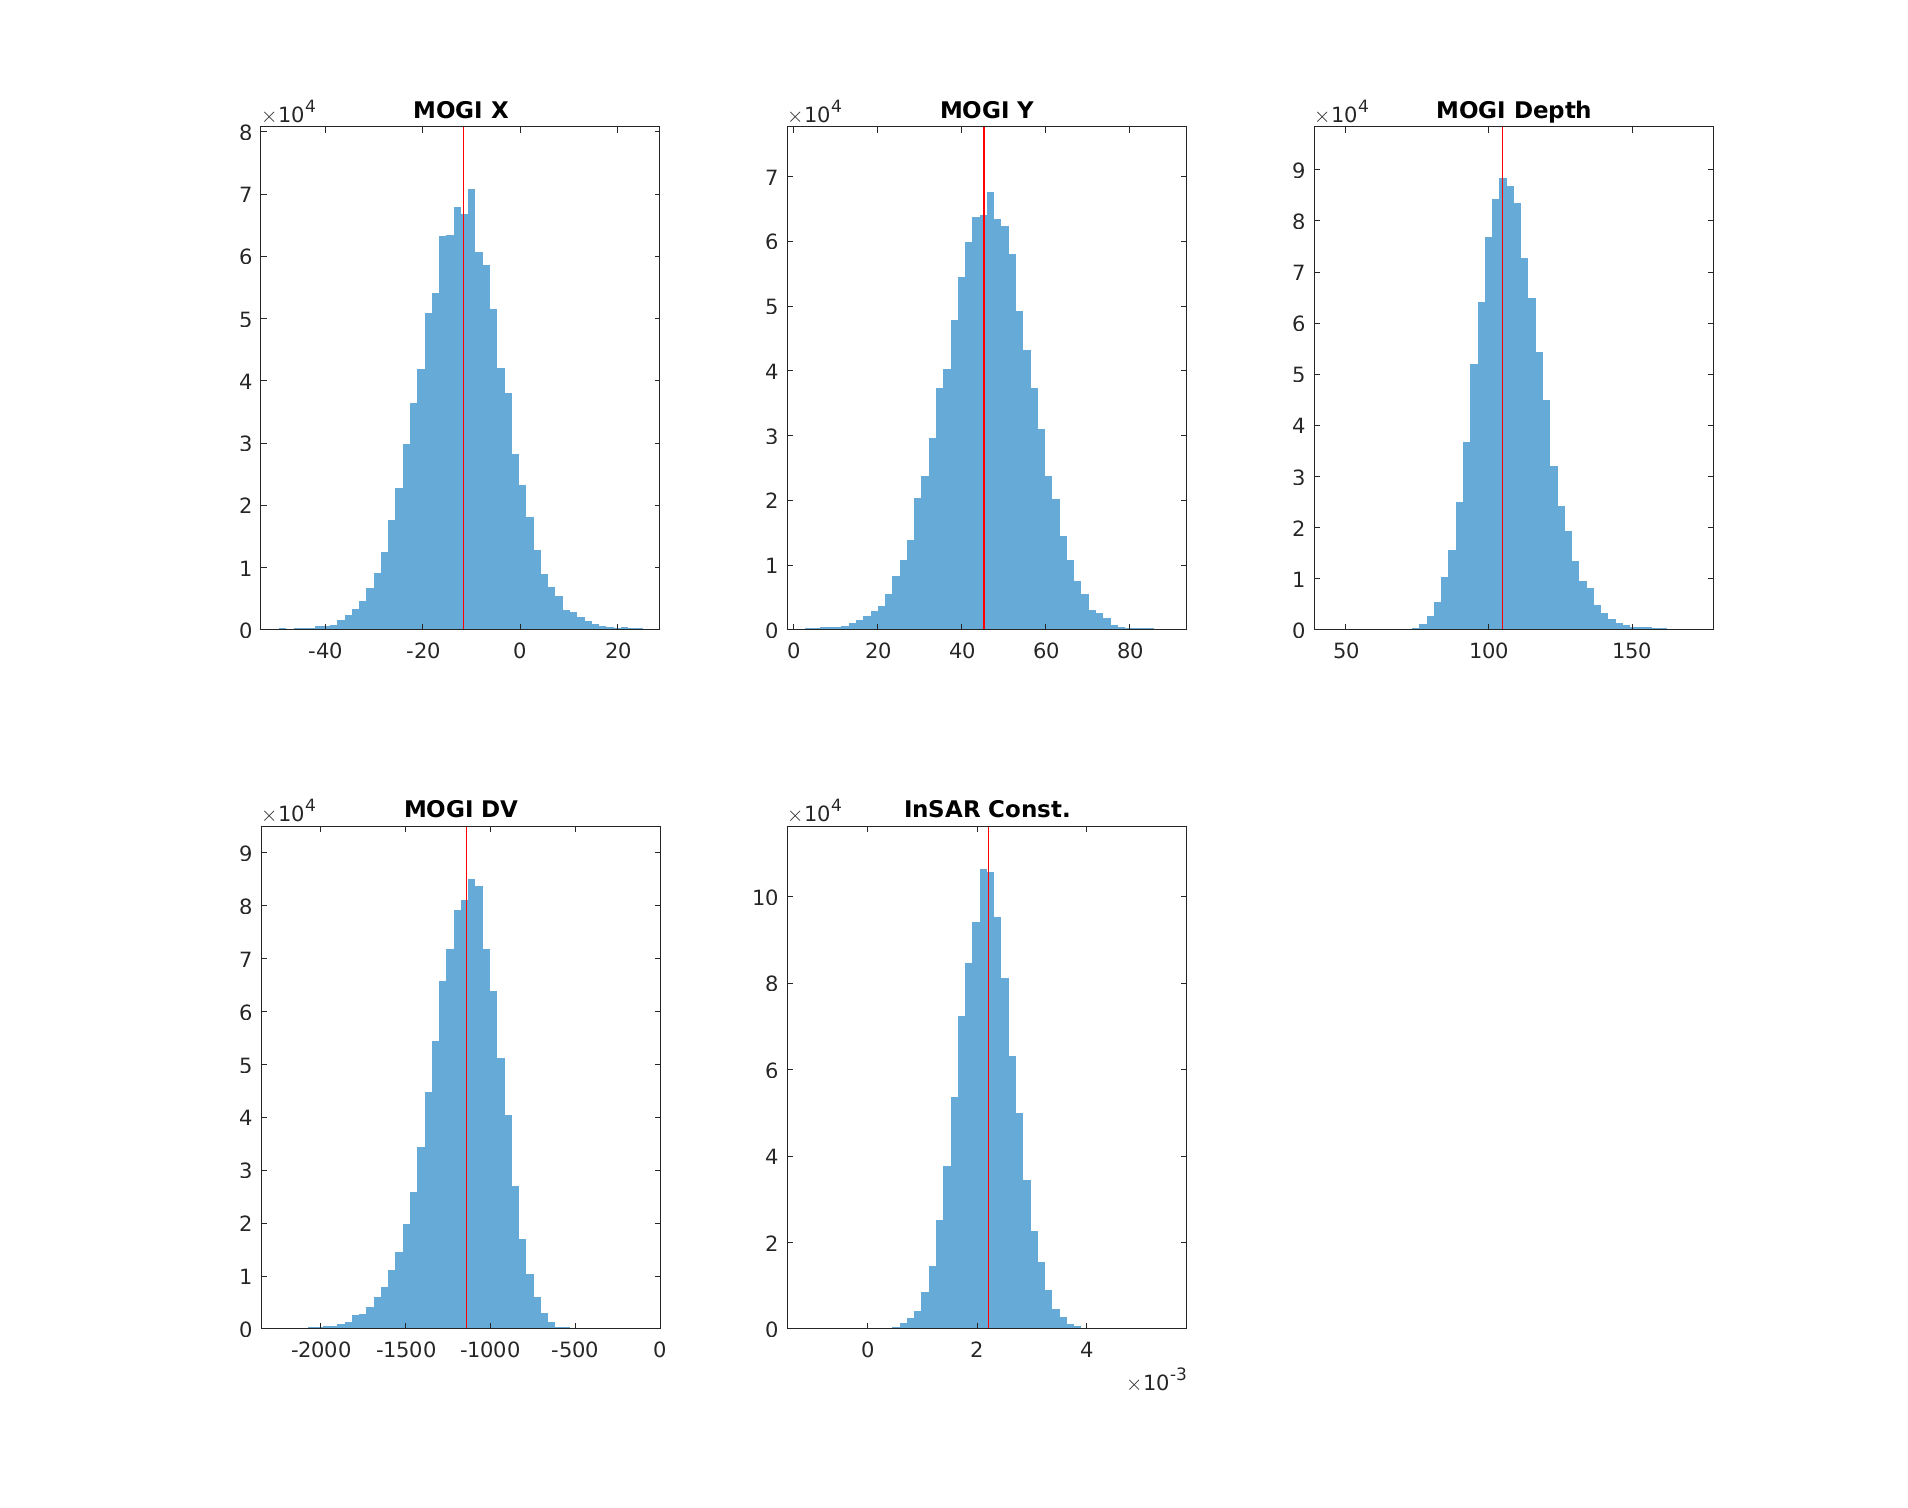
\includegraphics[width=1.0\textwidth]{PDFs.eps}
    \caption{反演参数的后验概率分布}
    \label{fig:pdf}
\end{figure}
原始形变数据,反演参数理论行便和二者的差见图\ref{fig:residual}。
\begin{figure}[htb]
    \centering
    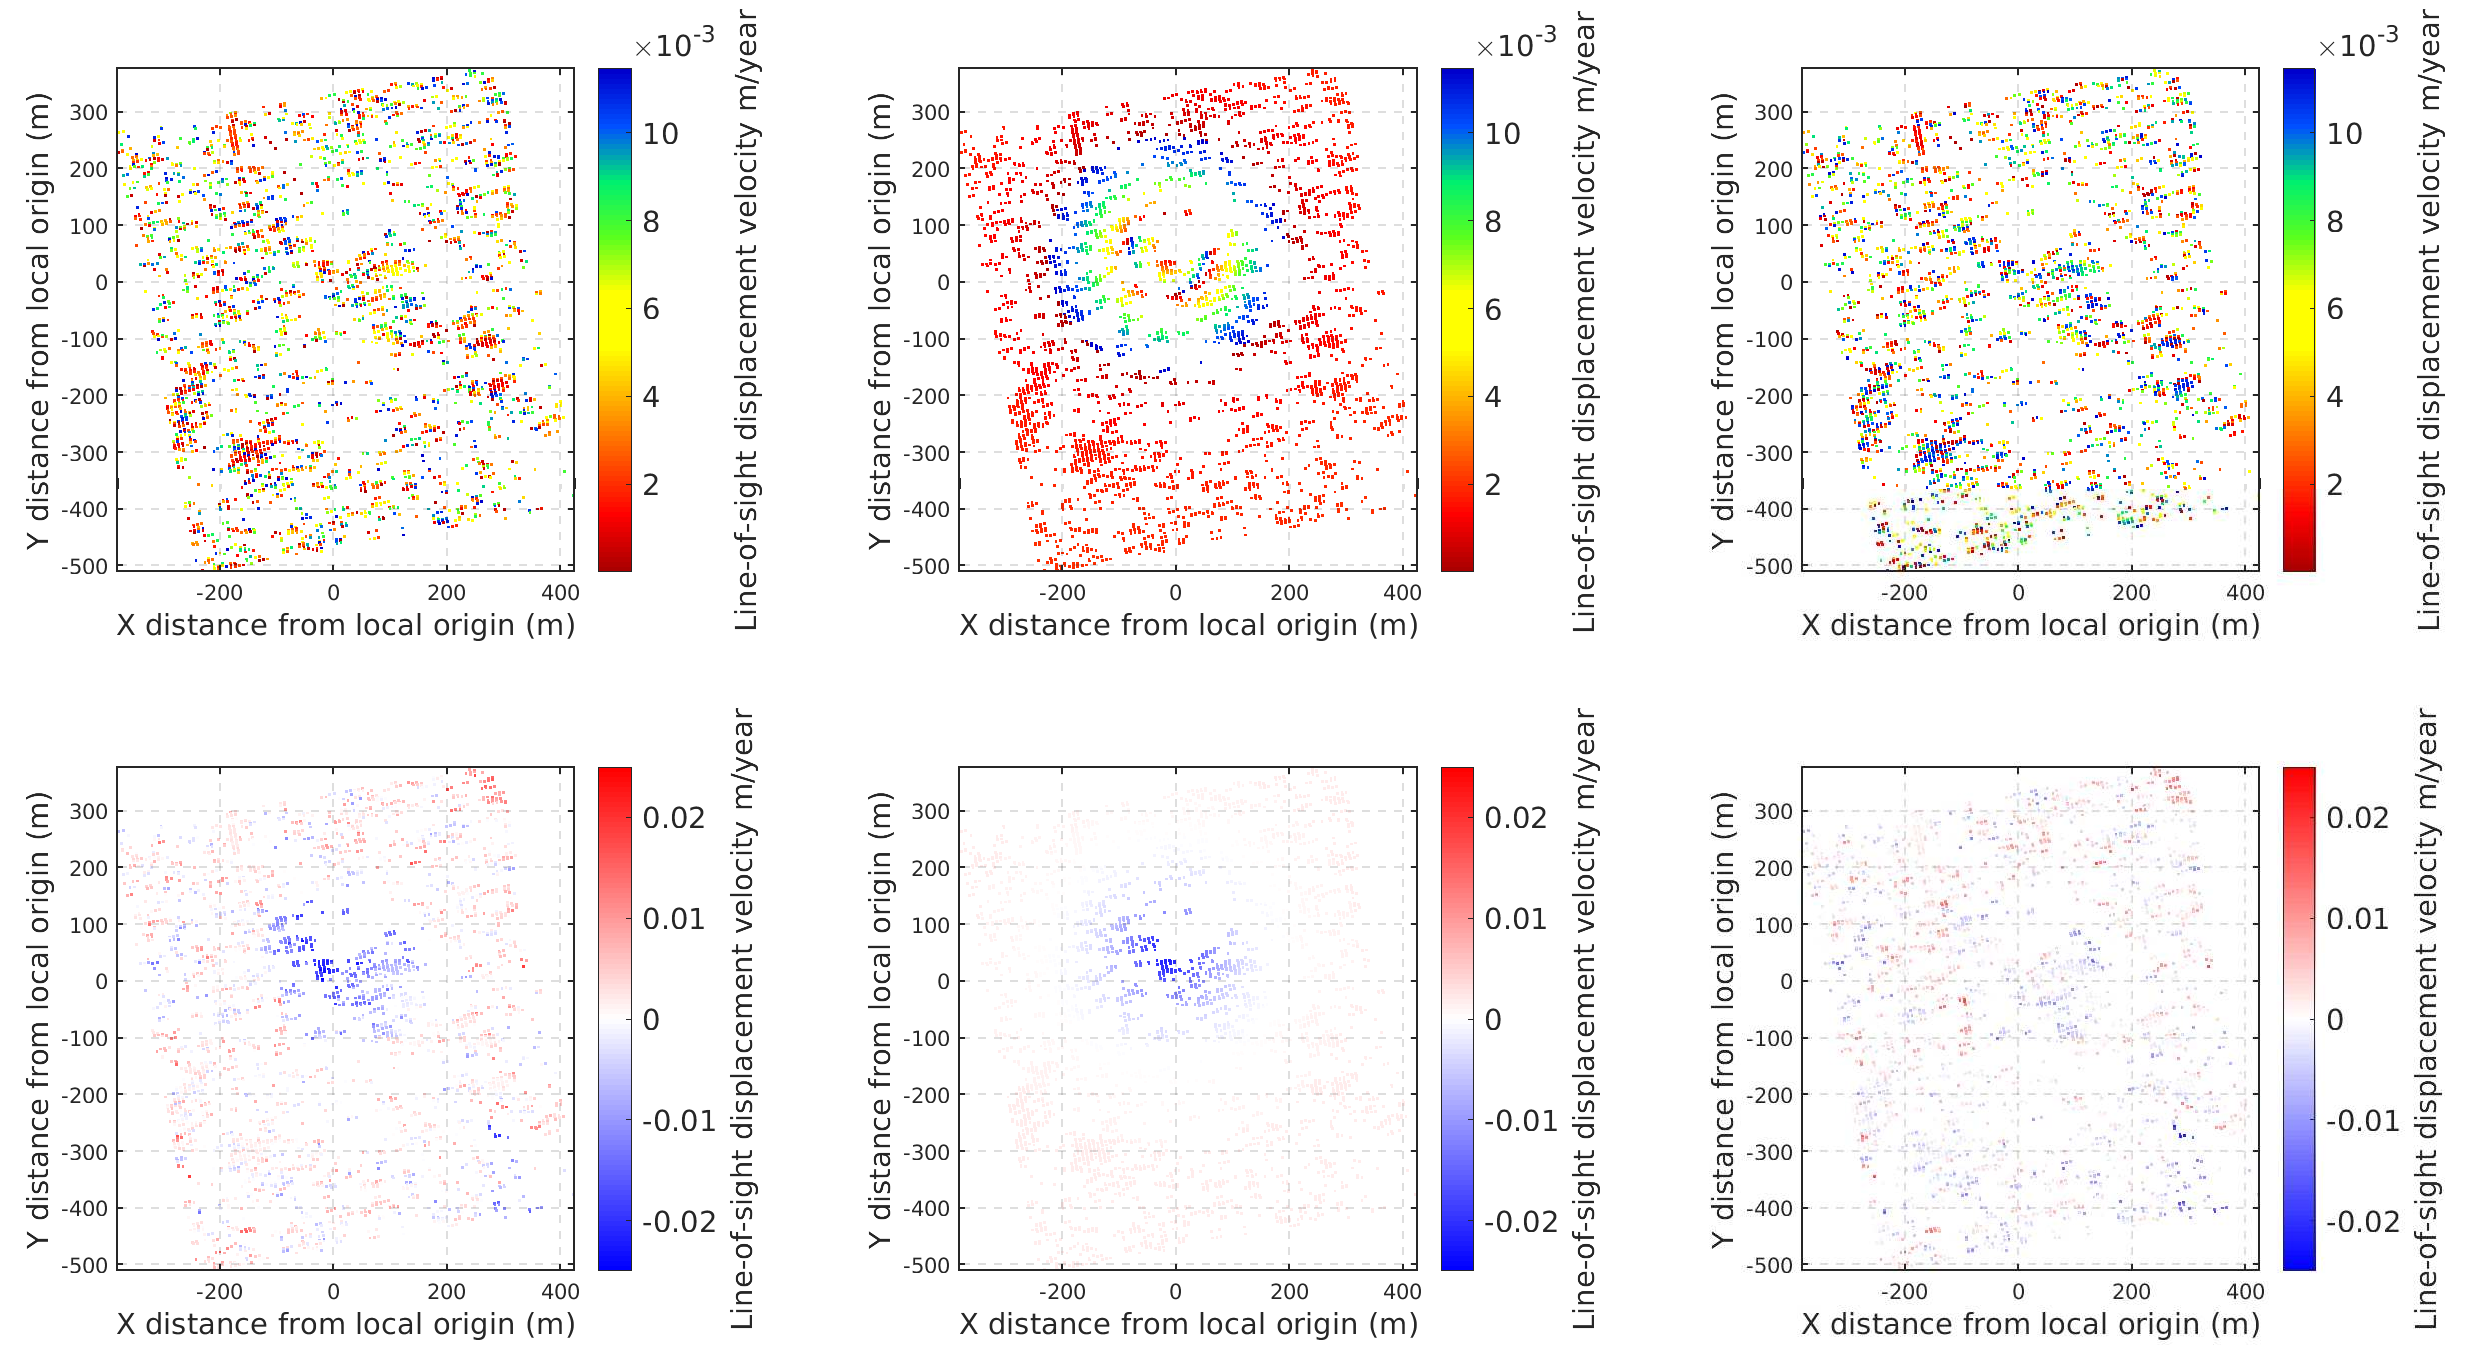
\includegraphics[width=1.0\textwidth]{croppedResidual.pdf}
    \caption{原始形变数据,反演参数理论形变以及二者的差}
    \note{注:六副图中,上面三副为未解缠的数据,下面三副为解缠之后的数据;
    左边的图为原始形变的数据,中间的图为模型理论推导的形变数据,右边为原始数据减去理论数据的剩余数据。}
    \label{fig:residual}
\end{figure}
从图\ref{fig:residual}来看,反演比较成功,模型反推的结果和InSAR观测的结果吻合得比较好。
但从图中可以看出,InSAR的结果仍有很多不吻合的地方。
一方面,可能是数据处理的原因,本研究分析的区域较小,大概在1平方公里左右,
所得到的PS点也不够密集,不一定能比较全面地覆盖当地的所有形变特征。
另一方面,也有可能是模型较为粗糙的原因,mogi模型是比较简单的模型,
可能实际导致形变的扰动源比较复杂。
从图\ref{fig:residual}中的剩余形变图可以看出,该区域的下半部分有不太明显的下沉,上半部分有一定的上升,
这部分的形变没有被mogi模型解释,如果采用更精确的模型,可能会有更好的反演效果。

\section{与其他研究成果的比较}
由于本研究的研究区域在carlsbad市区,和两条重要的高速公路相邻,一旦坍塌会造成相当大的损失。
所以,当地政府组织相关专业人员对此地进行了详尽的调查。

2009年,某一二维地震反射评估给出了该卤水井内部的空洞的大概形状。
空洞的中心在尤金妮娅1号钻井处,近似呈梨型,北部较窄,南部较宽。
2011年又开展了该处高分辨率大地电磁调查,研究发现此区域地下有较明显的低阻区。
低阻区向北延伸至285和62-180两条高速公路,向南延伸至CID南方运河。
这是该区域地下空洞的有效证明。
此后,当地相关部门和公司通过诸多手段得到了地下空洞的详细分布,并于2018年9月展开空洞填补工作。
从有关部门给出的地下空洞的详细信息来看,本研究所建的模型中扰动源的X,Y位置比较精确,
但深度差距比较大,模型中深度为地下103m,但实际的空洞在140m到180m之间。
深入差距比较大的原因应该是所用的mogi模型导致形变和实际空洞导致形变的物理原理上有一定的差异,
如果采用更准确的空洞模型应该会有更好的反演结果。

比较以上工作和InSAR的成果,可以得到以下结论。
\begin{enumerate}
    \item InSAR在此类问题中能起到一定的作用,InSAR能比较精确地估计出沉降区域的位置和大小。
    \item InSAR和地震,大地电磁方法相比,要节约很大的成本。
    \item InSAR能得到地表的变形数据,在坍塌预测方面有不可替代的作用。
    \item 和地震,大地电磁方法相比,InSAR方法无法得到精确的空洞形状等信息。
\end{enumerate}
\chapter{总结与展望}
本文首先阐述了InSAR技术的相关原理,然后利用ALOS PALSAR的数据
将SBAS-InSAR技术应用于新墨西哥州卤水井沉降的监测与建模上,
揭示了该卤水井沉降的情况。
验证了SBAS-InSAR方法在解决此类问题上的有效性。
之后利用沉降的数据对当地地下区域做了理论建模,得到了比较准确的模型。
能够对此形变给出比较有说服力的解释。
与其他研究成果相比,更突出了本研究使用的方法的准确性。

本研究的不足之处主要有以下几点:
\begin{enumerate}
    \item 研究区域较小,数据量不足,反演的结果准确性不高。
    \item 本研究只做了最简单的点源模型,和实际情况出入较大,采用和实际空洞更贴近的模型效果应该会更好。
\end{enumerate}

传统的地表形变监测方式成本较高,且数据量少,监测的精度也达不到要求。
InSAR作为一种的监测技术,成本低且精度足够高,是未来应当大力推广的监测方式。

中国是个资源大国,自然资源的开采很有可能带来一些次生灾害。
大规模的城市建设也同样有可能导致地面的沉降。
事实证明,InSAR是监测有地表形变征兆的灾害的很好的方法,
可以为地质灾害评估以及制定对应的政策提供数据支持。
% \input{chapters/floats.tex}
% \input{chapters/math.tex}
% \input{chapters/citations.tex}

\backmatter
%\bibliographystyle{ustcthesis-numerical}  % 顺序编码制
%\bibliographystyle{ustcthesis-authoryear} % 著者出版年制
\bibliographystyle{ustcthesis-bachelor}   % 本科生参考文献的格式
\bibliography{bib/bachelorthesis}

\appendix
%% !TeX root = ../main.tex

\chapter{补充材料}


\section{补充章节}

补充内容。


% \input{chapters/publications.tex}

\end{document}
